\documentclass[a4paper]{article}
\usepackage[english]{babel}
\usepackage[utf8]{inputenc}
\usepackage[margin=2.5cm]{geometry}
\usepackage{amsmath}\usepackage{amsthm}
\usepackage{amsfonts}
\usepackage{amssymb}
\usepackage[usenames,dvipsnames]{xcolor}
\usepackage{graphicx}
% \usepackage{tikz}
\usepackage[hidelinks]{hyperref}
\usepackage[autostyle]{csquotes}
\usepackage[backend=biber]{biblatex}
\usepackage{siunitx}
\usepackage{caption}
\usepackage{float}
\usepackage{subfig}
\usepackage{booktabs}
\usepackage{multirow}
\usepackage{graphicx}


% *** Manage the bibliography ***
\addbibresource{references_assignment_2.bib}

% *** Adjust the captions ***
\captionsetup{format=hang,labelfont={bf}}


\title{
	\large 
	\textsc{Lule\aa~University of Technology\\[5pt] 
		Predictive Analytics} \\[10pt]
	\rule{\linewidth}{0.5pt}\\
	\vspace{0.3cm}
	\Large Assignment 2\\
	\vspace{0.3cm}
	\huge \bf Replication study\normalsize
	\vspace{0.3cm}
	\rule{\linewidth}{0.5pt}  \\
}
\author{Alghisi Giovanni Angelo}
\date{\normalsize \today}

\begin{document}
	
	% *** Adjustment of autoref ***
	\renewcommand{\tableautorefname}{Tab.} % PS
	\renewcommand{\figureautorefname}{Tab.} % PS
	
	\maketitle
	
	\begin{abstract}
		In this report the results obtained replicating the study \cite{article:muller} will be discussed. In particular, the emulation has been developed by means of \textsc{RapidMiner}. This very powerful tool slightly differs from the ones exploited by \citeauthor{article:muller}; for this reason, and for others that will be presented throughout this essay, the outcomes deviate from the original ones, but allow to present the knowledges that have been acquired during the development of this assignment. 
	\end{abstract}
	% {\bf Keywords:} enter, keyword, here.
	
	\tableofcontents
	
	
	\section{Some words for the developed software}
		In this section the structure of the software developed in the \textsc{RapidMiner} environment will be described.\footnote{The software is available at~\cite{repo:pa-assignment-2}.} In particular, by describing the software components it will be possible to depict the reasoning above which the entire analysis lies, pinpointing the differences between this replica and the original study in terms of \emph{data preparation} and \emph{modelling}. For convenience, a subsection will be reserved to each process prepared, but please refer to the comments spread throughout the code itself for further information.
		
		\subsection{Opening data}
		 	The first process to be run is \verb|1a-opening_data|, that converts the provided \verb|.json| dataset into an \verb|ExampleSet|;\footnote{For this analysis it has been used the dataset available on Canvas and provided by Prof.~Jaap van de Beek and Prof.~Yomn Elmistikawy.} this is the starting point of the entire analysis in \textsc{RapidMiner}.
		 
		 \subsection{Filtering and preparing the data}
		 	The purpose of the task \verb*|2-filtering_and_preparing_data| is to clean the dataset, filtering it, and to prepare the data for the text preprocessing phase.
		 	
		 	As discussed in \cite{article:muller}, to increase the reliability of the analysis, all the reviews with less than two helpfulness ratings should be removed. Moreover, the process generates the following new features:
		 	\begin{itemize}
		 		\item \verb*|helpfulness| the \emph{target feature} obtained evaluating the ratio of the number of positive helpfulness ratings over the total amount of helpfulness feedbacks (per each review); if this ratio is above 0.5, then the feature assumes \verb*|true| value, otherwise \verb*|false|.
		 		\item \verb*|text_corpe|, obtained by the concatenation of review summary and the text itself. It is important to highlight that \citeauthor{article:muller} are a little bit vague, because they talk about ``the corpus'' of the reviews; for this replica it has been decided to consider both the summary and the actual text of each review.
		 		\item \verb*|text_corpe_length|, calculated by counting the number of words in the \verb*|text_corpe| feature. 
		 	\end{itemize} 
	 	
	 	\subsection{Preprocessing the text}\label{subsec:processing-the-text}
	 		This phase is crucial to sensibly apply the \emph{LDA} algorithm, as it consists of filtering the noise as much as possible from the text to be processed. Thus, \verb*|3b-processing_text| deals with the following sequence of operations:
	 		\begin{enumerate}
	 			\item \emph{converting all characters to lower-case};
	 			\item \emph{tokenizing} each \verb*|text_corpe| occurrence into single words;
	 			\item \emph{removing stop words}, that is to delate uninformative but frequent words. Actually, the stop words can be classified in two different families:
	 			\begin{itemize}
	 				\item \emph{standard stop words}, and for this particular study the only English stop words have been considered, like ``the'', ``and'' or ``I''; this has been done by means of pre-implemented primitives, available in \textsc{RapidMiner};
	 				\item \emph{custom stop words}, related to the main topic of our analysis (i.e.~video games reviews), like ``game'' or ``play'';
	 			\end{itemize}
 				\item \emph{stemming}, an operation that consists of reducing a word to its stem, like the words ``analyze'' and ``analysis'' to ``analy''; in particular, the \emph{Snowball algorithm} has been used.\footnote{Not knowing in deep the distinctions that different stemming algorithms present, for this work it has been chosen the most suggested by the \textsc{RapidMiner} community.}
	 		\end{enumerate}
 			At this point a clarification is required: the original study performed by \citeauthor{article:muller} relies on the exploitation of the \emph{Lemmatizing} algorithm. This means that words like ``dog'', ``Dog'', ``dogs'', and ``Dogs'' would all change to ``dog'' (word are transformed into its dictionary form). The lemmatizing approach is, without any doubt, more gentle, but, due to the fact that \textsc{RapidMiner} does not provide this algorithm, stemming has been exploited instead, as suggested by the community itself. 
	 		
 		\subsection{Preparing video games stop word list}
		 	The list preparation of custom stop words is carried out with \verb*|3a-preparing_videogame_stopword_list| process, in order to handle a possible problem that could arise. The Stem algorithm is applied to \verb*|review_corpe| text. This causes the words to be truncated (e.g. ``games'' could become ``game''). Thus, if the stop word list include just the word games (without ``game''), it will be useless to filter the \verb*|review_corpe| text considering it, because the Stem algorithm prevents it to appear in the output (maybe ``game'' would arise there, or again ``gam'', but this words differ from ``games''). In order to improve the robustness of our analysis, the list has been produced applying the same Stem algorithm to the words specified by the user through a \verb*|.txt| file. In this way, the mechanism is more robust and easier to be used.
		 	
		 \subsection{LDA execution}
		 	The process \verb*|3c-LDA_execution| does exactly what the name suggests: by means of an already-arranged function, it is possible to recognise topics using the LDA method. The algorithm has been tuned to search for 100 topics and consider 10 words per each one.
		 	
		 	Considering these results, the dataset has now, in addition to \verb*|overall| and \verb*|text_corpe_length|, 100 new descriptive features consisting in the probability of each instance to belong to the related topic.\\
		 	What about the list of 10 words per topic, it has been used to entitle each topic itself in order to simplify the result analysis.
		 	
		 \subsection{Building and evaluating the Random Forest}
		 	Finally, by means of \verb*|4-building_random_forest|, it is possible to train and evaluate the \emph{Random Forest} algorithm. 
		 	
		 	As suggested by the article, the dataset has been split as follow:
		 	\begin{itemize}
			 	\item 80\% of the instances for the \emph{training set};
			 	\item 20\% of the instances for the \emph{testing set}.
		 	\end{itemize}
	 		Considering that the \emph{stratified sampling} approach is not required in this case, the \emph{random sampling} technique has been preferred over the \emph{linear sampling} one in order to avoid the risk of introducing bias. Indeed, due to the fact that the ordering problem of instances has been neglected, linear sample could lead to negative results.
	 		
	 		\textsc{RapidMiner} allows the user to deeply tune the random forest algorithm; the main choices taken for this study are the followings:
	 		\begin{itemize}
	 			\item as \citeauthor{article:muller} have done, a model consisting of 128 trees trained on bootstrapped sub-sets of the \emph{training set} has been used (\emph{bagging}); the prediction strategy chosen in case of dissenting tree model predictions is the \emph{confidence vote} one, thus the class that has the highest accumulated confidence.
	 			\item the \emph{Gini-index} measure of impurity has been selected \emph{to make the trees grow}, in accordance to \citeauthor{article:muller};
	 			\item a variety of \emph{prune} techniques can be exploited, in order to prevent the predictive model to overfit the training set; the only strategy applied in this context during the present project has been to set the \emph{maximal depth} parameter to 10, in order to limit the depth of each random tree.
	 		\end{itemize}
 		
			The performances of the model can then be evaluated using the \emph{testing set}, and the output of this process consists in both the \emph{weight of each feature} and some performance indexes, like \emph{precision}, \emph{accuracy}, \emph{recall}, \emph{AUC} and \emph{ROC} plots.		
			
		\begin{figure}[p]
			\centering
			\subfloat[]{
				\centering
				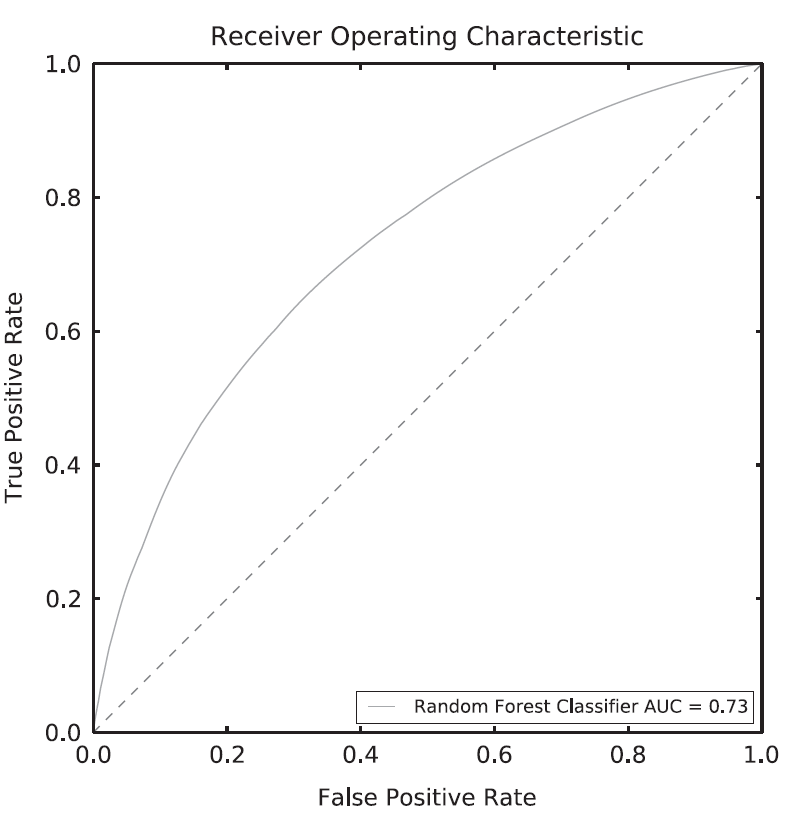
\includegraphics[height=0.475\linewidth]{Images/muller_roc}
				\label{fig:muller_roc}
			}
			\quad
			\subfloat[]{
				\centering
				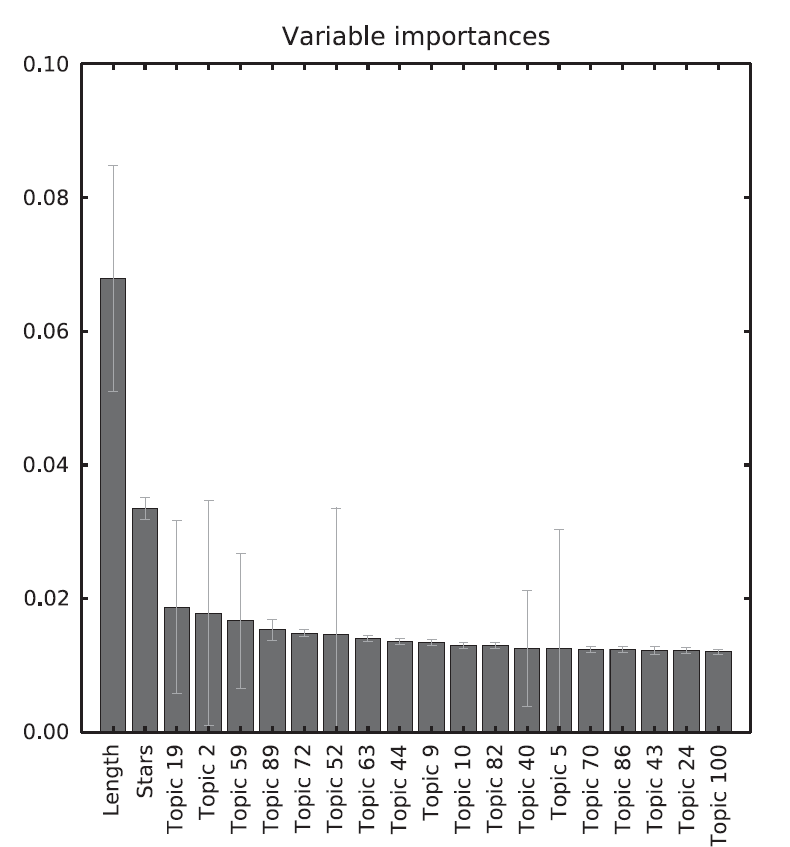
\includegraphics[height=0.475\linewidth]{Images/muller_topic_weights}
				\label{fig:muller_topic_weights}
			}
			\caption{Results obtained during this study.}
			\label{fig:muller_results}
		\end{figure}
		
		\begin{figure}[p]
			\centering
			\subfloat[]{
				\centering
				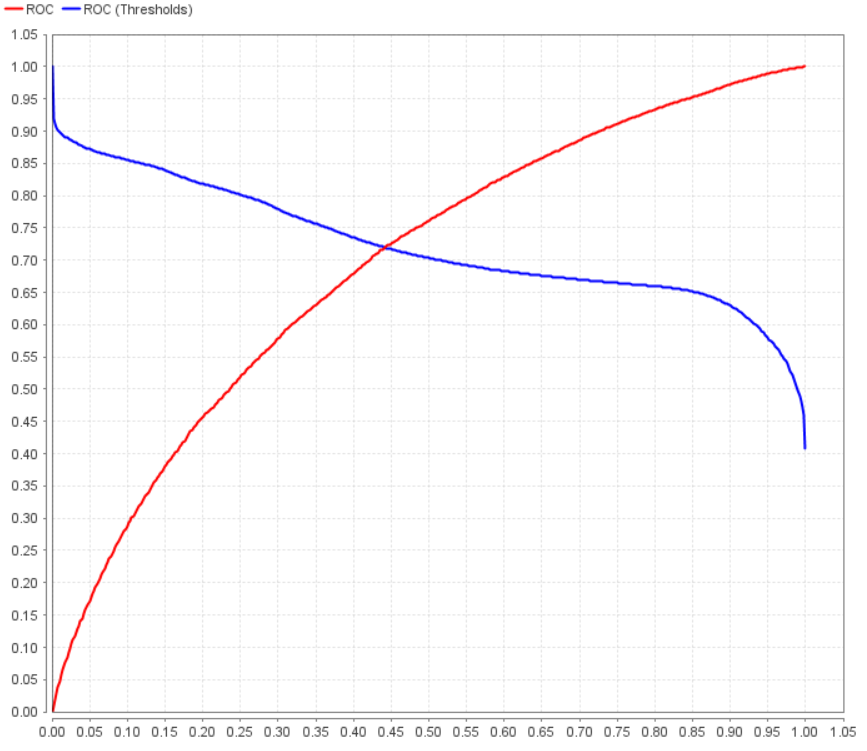
\includegraphics[height=0.43\linewidth]{Images/my_gini_index_roc}
				\label{fig:my_gini_index_roc}
			}
			\quad
			\subfloat[]{
				\centering
				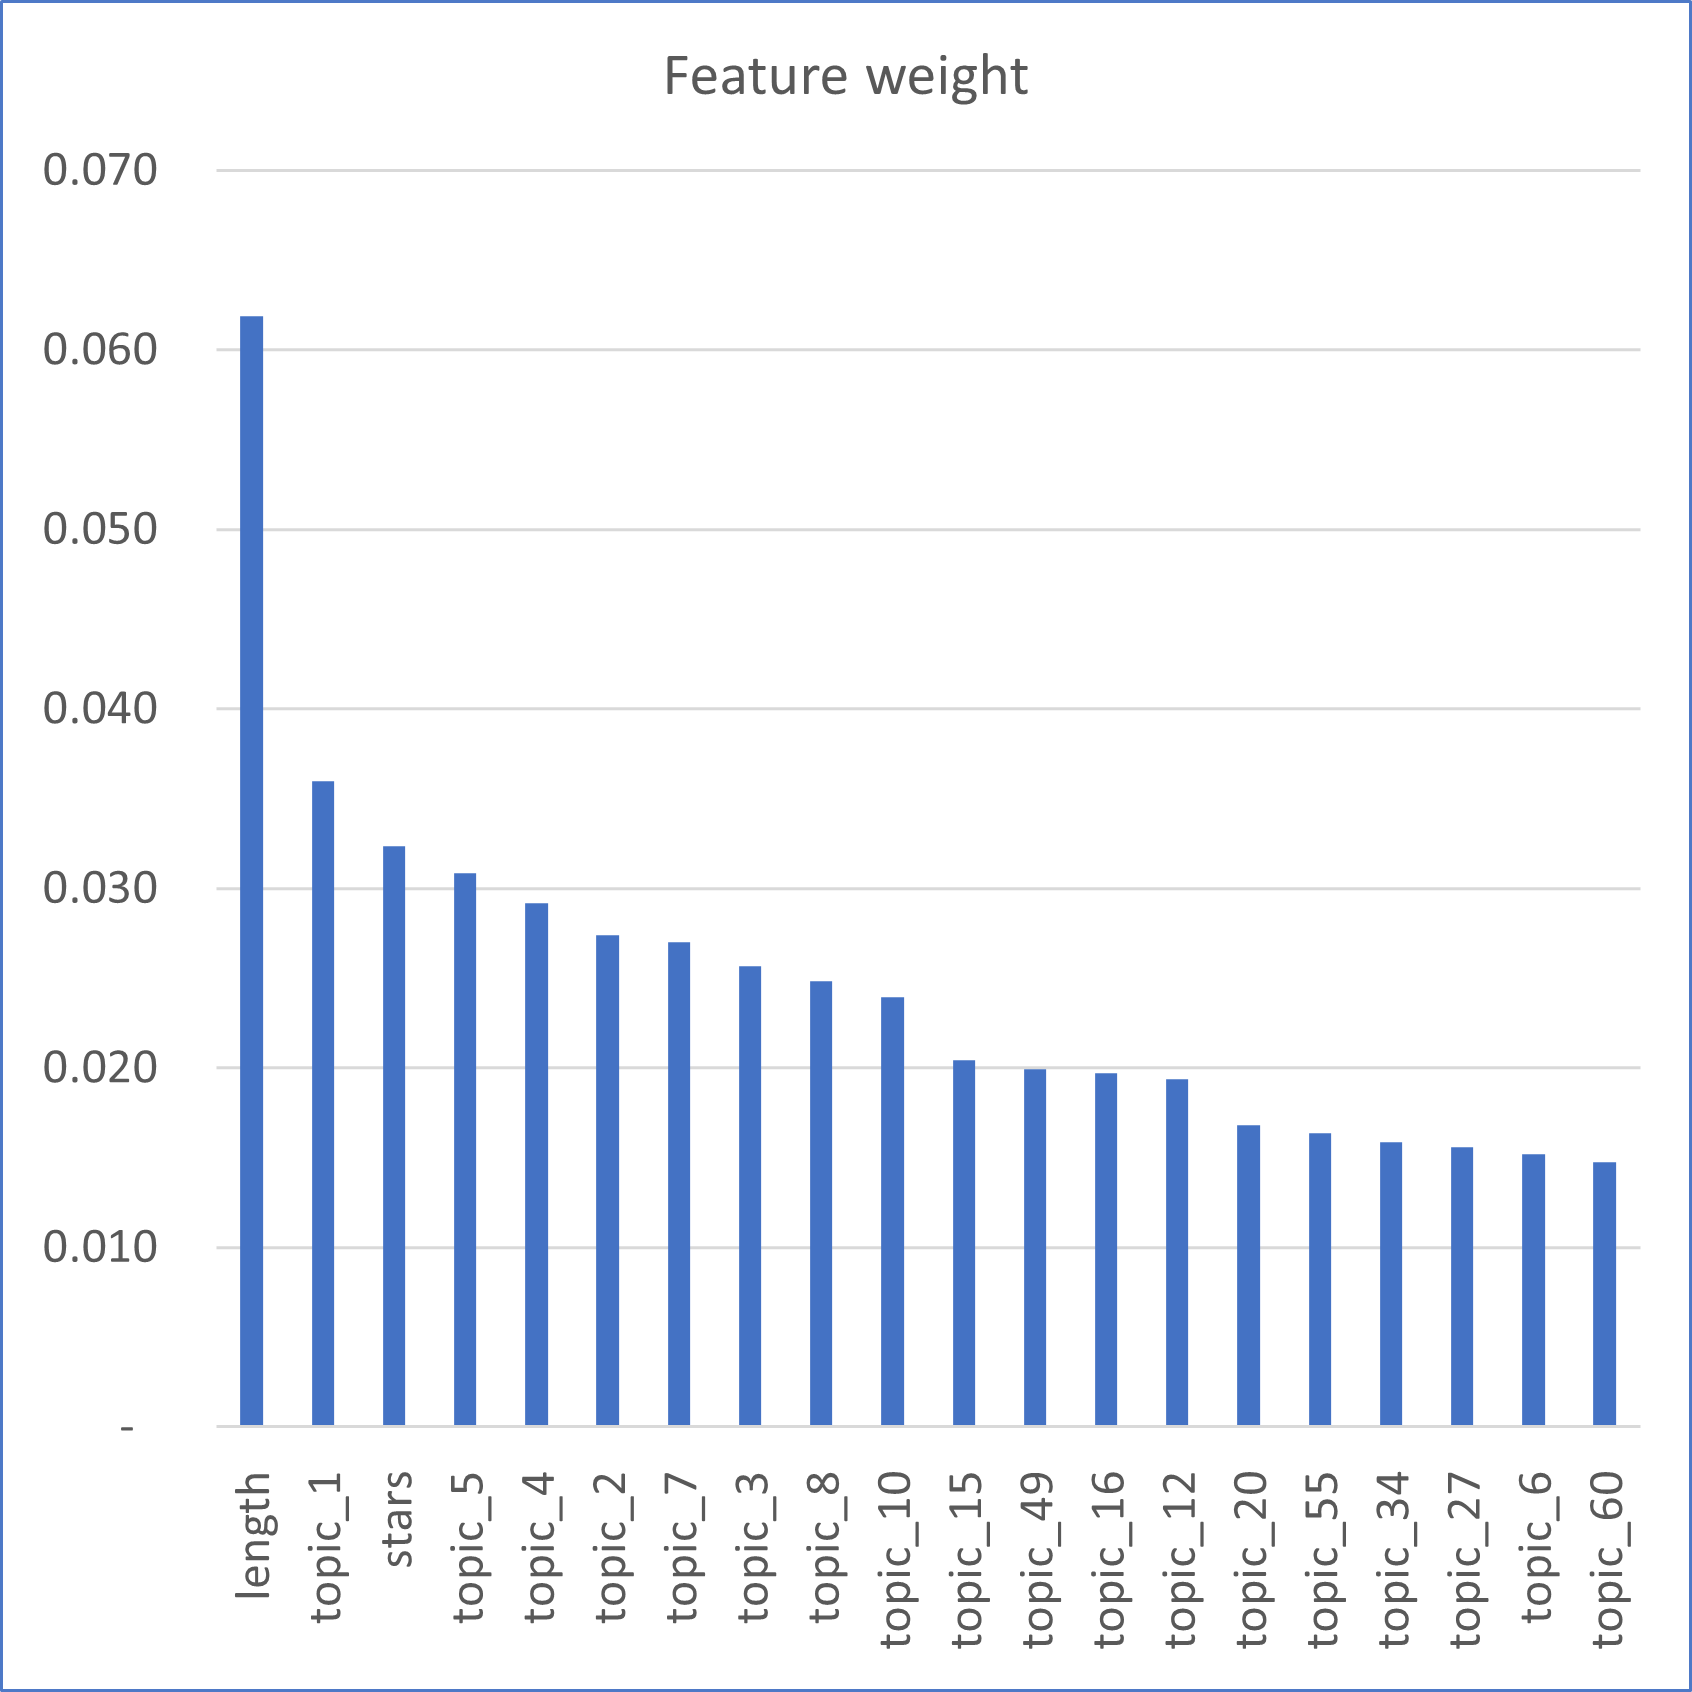
\includegraphics[height=0.43\linewidth]{Images/my_topic_weights}
				\label{fig:muller-results}
			}
			\caption{Results obtained during this study.}
			\label{fig:my_results}
		\end{figure}
	
		 			 	
	\section{Results}
		\subsection{The main performance indexes}
			The time comes to analyse the results obtained testing the model developed. As first index, we can consider the \emph{accuracy}, calculated directly in \textsc{RapidMiner}: the value of 77.48\% results, and this means that the model is able to guess the correct value of the target feature about 77.5 over 100 times.
			However, even if this seems a good result, is necessary to partially consider this achievement.
			
			The final dataset (used both to train and test the model) is indeed imbalanced: there are 362,246 positive helpful reviews, and 106,934 negative ones. This, considering also the fact that accuracy does not take into account the cost of an incorrect prediction, could lead to prefer a different metrics to gauge the performances of the resulting model. Often the \emph{AUC} index, i.e. the Area Under the ROC Curve, is more sensible, as it can be viewed as a measure of \emph{separability}. Lets thus consider Figure\autoref{fig:my_gini_index_roc} and compare it with the ROC curve obtained by \citeauthor{article:muller}. The AUC got is 69.2\%, slightly less than the one of the authors (73\%).
			
			However, the \emph{best} parameter does not exist: the designer of the model should always consider the purpose of it. If, for instance, the model was developed by \textsc{Amazon} to rank the reviews to select and propose them to people visiting the e-commerce, than the primary goal would be to pick out \emph{only} the helpful reviews. In this situation, the model should be taken in order to maximise its \emph{precision}, i.e. the fraction of positive predictions that are actually positive (in terms of helpfulness). Indeed, the main aim of the company would not be to choose a model able to correctly distinguish all the good reviews from the bad ones (supposing that the pool of available reviews is wide enough), but to propose the purchaser less useless reviews as possible. In this cases comes in hand the \emph{confusion matrix} (\autoref{tab:confusion_matrix}), and in particular the positive class of precision, which its value is of 77.54\%.\footnote{The value of accuracy and positive class precision are very close due to the fact that the dataset is imbalanced and most of the reviews are helpful.}
			
		\begin{table}[]
			\centering
			\caption{Confusion matrix obtained during study.}
			\label{tab:confusion_matrix}
			\begin{tabular}{@{}cl|cc|c@{}}
				\toprule
				\multicolumn{2}{c|}{}             & True false & True true & Class precision \\ \midrule
				\multicolumn{2}{c|}{\multirow{2}{*}{Pred.~false}} & \multirow{2}{*}{224}   & \multirow{2}{*}{139}   & \multirow{2}{*}{61.71\%} \\
				\multicolumn{2}{c|}{}             &            &           &                 \\
				\multicolumn{2}{c|}{\multirow{2}{*}{Pred.~true}}  & \multirow{2}{*}{20994} & \multirow{2}{*}{72479} & \multirow{2}{*}{77.54\%} \\
				\multicolumn{2}{c|}{}             &            &           &                 \\ \midrule
				\multicolumn{2}{c|}{Class recall} & 1.06\%     & 99.81\%   &                 \\ \bottomrule
			\end{tabular}%
		\end{table}
			
		\subsection{Variable importance}
			As stated in the article, random forest algorithms are very obscure and cryptic, preventing the person who implemented them to find the comprehensible relationship between the describing features and the target one. However, some insight can be given by the analysis of weights possessed by each descriptive feature. Lets thus consider and compare Fig.\autoref{fig:my_gini_index_roc} and Fig.\autoref{fig:muller_topic_weights} which show the impact of the twenty most affecting attributes. The first thing that can be noticed is the (relative) big weight of the \verb*|review_corpe_length|; both the models show that the longest the review, the most helpful it is. For what concerns the others, it is very difficult to do comparisons because this work relies on several different decision taken with respect the ones of \cite{article:muller}, like the exploitation of the stemming algorithm instead of the lemmatizing one. However, something can be done observing \autoref{tab:topics_list} and Tab.~\ref{fig:mullertopiclist}, which shows the ten most probable words ordered by probability. The list reveals that the most impactive reviews deal with:
			\begin{itemize}
				\item overall affective judgements (e.g., 8, 49, 16, 34, 27, 60);
				\item comments related to the quality of the graphics, extra options or controllers(e.g., 10, 55, 6);
				\item topics related to specific audiences (e.g., 7);
				\item plot of the story (e.g., 4);
				\item the video game series itself (e.g., 1, 2, 3);
				\item if the game has been suggested by a friend of the reviewer (e.g., 5);
				\item quality of the service provided by \textsc{Amazon} (e.g., 15).
			\end{itemize}
		
			Even if the ten words per each topic differ from the ones obtained by \autocite{article:muller}, it is possible to find some common denominator in terms of interpretations of the argument treated. Another possible source of deviation, further the ones discussed in the \autoref{subsec:processing-the-text}, can be found in the number of iterations of the LDA algorithm. For this work it has been chosen to limit this parameter to 1000;\footnote{This number has not been selected directly, but used the one suggested by \textsc{RapidMiner}.} however, the number selected by the authors is not clear, due also to the fact that the links to the source code provided by the article are no longer working, so it has not been possible to analyse it.
			
	 	
			
		\begin{figure}[p]
			\centering
			\caption{Topic list of the eighteen most relevant topics obtained by \citeauthor{article:muller}.}
			\label{fig:mullertopiclist}
			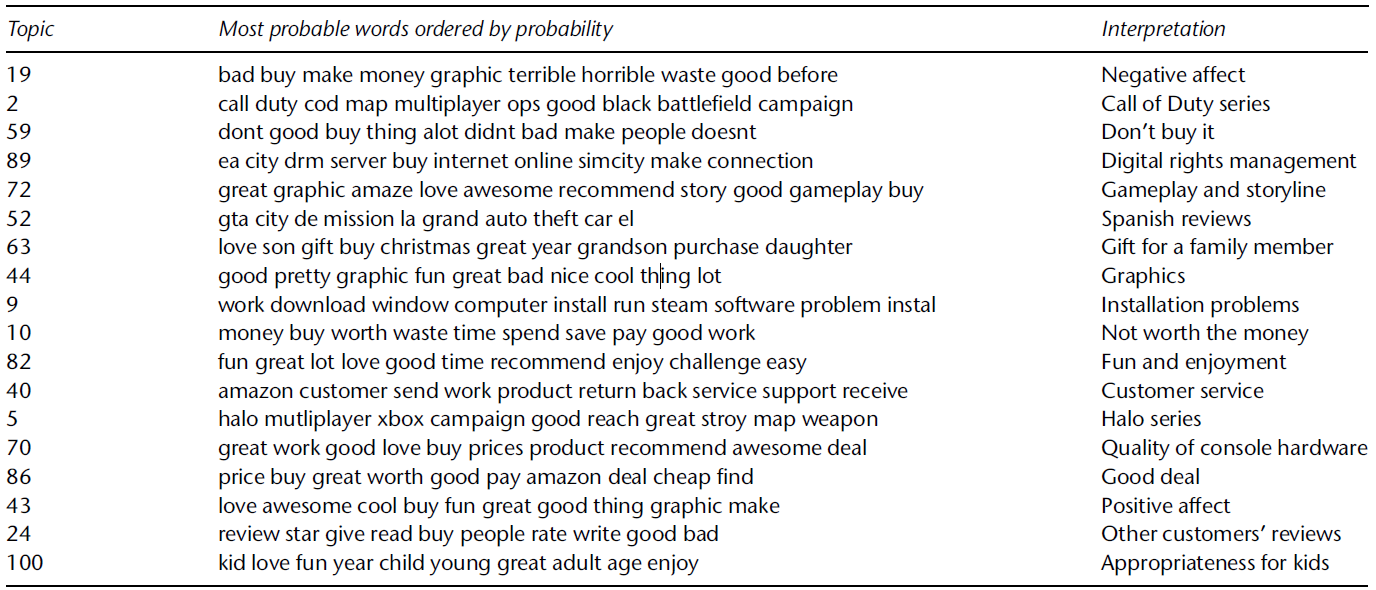
\includegraphics[width=1\linewidth]{Images/muller_topic_list}
		\end{figure}
		
		\begin{table}[p]
			\centering
			\caption{Topic list of the eighteen most relevant topics obtained during this study.}
			\label{tab:topics_list}
			\resizebox{\textwidth}{!}{
				\begin{tabular}{lll}
					\toprule
					\textbf{Topic} & \textbf{Most probable stems ordered by probability} & \textbf{Interpretation} \\
					\midrule
					1  & sim expans pack hous make build creat get stuff lot & The Sims series \\ 
					5  & peopl say know think review want whi thing get make & Game recommend by friends \\ 
					4  & stori charact scene voic act cut end movi gameplay plot & Plot \\ 
					2  & fallout oblivion quest skyrim max world bethesda scroll elder morrowind & The Elder Scrolls series \\ 
					3  & charact battl final fantasi rpg stori system rpgs time squar & Final fantasy series \\ 
					7  & love old year kid son bought great fun daughter christma & Game for children \\ 
					8  & get want thing make time good use peopl take find & Good review - general comments (1) \\ 
					10  & love great amaz awesom graphic buy get recommend perfect fan & Very good graphics \\ 
					49  & fun great lot recommend enjoy good love get time high & Good review - general comments (4) \\ 
					15  & amazon order product work ship purchas receiv item return box & Good service provided by Amazon \\ 
					12  & hour fun get time day bore got beat enjoy keep & Good review - general comments (7) \\ 
					16  & dont get buy good cant alot that thing say got & Bad review - general comments (3) \\ 
					55  & player allow featur option set abil addit system chang includ & Extra features and options \\ 
					20  & get time see look move run thing make head take & (???) \\ 
					34  & money buy wast time worth bought want spend worst piec & Bad review - waste of money \\ 
					27  & got work bought tri day went start buy thought came & Good review - general comments (3) \\ 
					6  & keyboard key use type light mous macro switch press usb & Review related to peripherals and controllers \\ 
					60  & good pretti get graphic bad great thing nice look lot & Good review - general comments (5)  \\ 
					\bottomrule 
				\end{tabular}
			}
		\end{table}
			
		
		\section{Final reflections}
			\subsection{Three things I have learned}
				\paragraph{What LDA is and how to preprocess the text accordingly} One of the most interesting topic I read about during the entire work has been the LDA algorithm. It would be very interesting to properly study how these algorithms work and the understand the basic language theory upon which they rely. I think that this is strongly coupled with the study of lemmatizing and stemming. Summary, during this work I had the possibility to touch these thematics, even if I am conscious that this is less than the tip of the iceberg.
			
				\paragraph{What is a confusion matrix}
				I have heard about this concept before, but I have never had a chance of trying to reflect on it in this way; the main problem is that there are a lot of different acronyms and terms (TP, TN, FP, FN, TPR, FPR, recall, precision, \dots) and at the first glance it is very easy to get confused and have difficulties at understanding the concepts behind it. 
				
				\paragraph{What are the 4Vs of Big Data} ``Big Data'' is a word that in some way has been included in the vocabulary of everybody, but I did not know the exact meaning; I was stuck at the general description given by television news. In my opinion, \cite{article:muller} is nice and sweet and reading it gave me the occasion, maybe not to master the concept itself, but at least to have a more rigorous idea of what are the 4Vs of Big Data and how many controversy affect the related fields of research.
				
			\subsection{Two questions I still have}
				\paragraph{How to obtain the ROC curve and why AUC is a mesure of separability} One of the biggest difficulties I had during the development of this project has been to understand what ROC is and how to calculate it. I know that the AUC is a measure of the separability capacity of the trained model, but I could not get the statistical theory behind it. I believe that, as discussed in the previous subsection, I have not assimilated the meaning of the several acronyms yet, and I should concede to myself a little bit more time to read about them carefully.
				
				\paragraph{Why I got more instances after the first filtering procedure} 
				In the article, \citeauthor{article:muller} assert that after having excluded reviews (from the original dataset) with less than
				two helpfulness ratings (in order to increase the reliability
				of their analysis), the resulting dataset consists of 495,358 video
				game reviews. However, after this first filtering procedure, I got 469,180 elements. I cannot figure out how this is possible, having checked the process several times.
				
			\subsection{What I enjoyed}
				The most exciting part of the entire work has been to exploit the LDA algorithm and have \emph{successfully} extracted actual topics from the reviews. I do not know the exactly reason, but to run the program and finally get the list of topics from all the reviews is very satisfactory, especially when you compare the ten most likely words and they make sense. Maybe they are not always accurate, or the topic cannot be understood, but what an achievement!
	\clearpage
	\nocite{*}
	\printbibliography 
		
\end{document}